\documentclass[b]{beamer}

\usepackage[french]{babel}
\usepackage[utf8]{inputenc}

\usepackage{graphicx}
\usepackage{amsmath,amsfonts,amsthm}

\usetheme{Warsaw}

\title{\texttt{Analyse Discriminate Linéaire}}
\author{HUYLENBROECK Florent, DELFOSSE Charly, JOSSE Thomas}

\begin{document}
	\begin{frame}
		\titlepage
	\end{frame}

	\begin{frame}
		\frametitle{Table des matières}
		\tableofcontents
	\end{frame}
	\section{Introduction}
	\begin{frame}
		\frametitle{Qu'est-ce que l'ADL?}
		Cette technique fait partie des techniques d'analyse discriminante prédictive. Le but et de pouvoir expliquer et prédire l'appartenance d'un individu à un groupe prédéfini à partir de caractéristiques qui ont été mesurées au préalable à l'aide de variables prédictives.
		On peut la comparer à la régression logistique. 
	\end{frame}
	\begin{frame}
		\frametitle{La règle bayesienne}
		Cette règle consiste à produire une estimation de la probabilité après notre affectation.
		Cela veut dire que nous devons réaliser une estimation pour une probabilité conditionnelle:
		\[
			P(Y = y_k | X) = \frac{P(Y = y_k) \times P(X| Y = y_k)}{\sum_{i=1}^{K} P(Y = y_i)\times P(X|Y = y_i)}
		\]
		
		Où $X$ contient les $j$ variables prédictives [$X = X_1,...,X_j$], $n$ est le nombre d'observations réparties dans $K$ groupe d'effectifs $n_k$, Y est notre variable à prédire qui prend des valeurs dans l'ensemble \{$y_1,...,y_K$\}. 
		Nous avons aussi $P(Y = y_k)$ qui est la probabilité d'appartenance à la classe $y_k$ et $P(X|Y = y_k)$ qui est la fonction de densité des x si par rapport à l'appartenance à la classe $y_k$.
	
		Et donc, ce qu'on recherche avec l'analyse discriminante (en général car il existe d'autres type d'analyse discriminante) est de trouver l'estimation de $P(X|Y = y_k)$.
	\end{frame}
	\section{Fonctionnement}
	\subsection{Principe géométrique}
	\begin{frame}
		\frametitle{Ce qu'on veut}
	\end{frame}
	\begin{frame}
		\frametitle{Développement}
		\begin{itemize}
			\item Chaque groupe d'observations remplacé par barycentre
			\item On trace une droite perpendiculaire au segment qui relie les deux barycentres
			\item L'intersection entre la droite tracée et le segment est appelé le point "zéro"
			\item Cette droite est placée en fonction des échantillons (s'ils sont équilibrés la droite est équidistante des barycentres, sinon celle-ci est plus proche du barycentre dont l'échantillon est le plus représenté).
		\end{itemize}
	\end{frame}

	\subsection{Principe statistique}
	\begin{frame}
		\frametitle{Ce qu'on veut}
		On veut replacer nos données dans un nouveau repère tel que les points sont le poche possible au sein d'un même groupe, mais ceux-ci doivent être aussi distants que possible entre les 2 groupes.
		
		$\Rightarrow$ Exemple aux slides suivantes.
	\end{frame}

	\begin{frame}
		\frametitle{Données de base}
		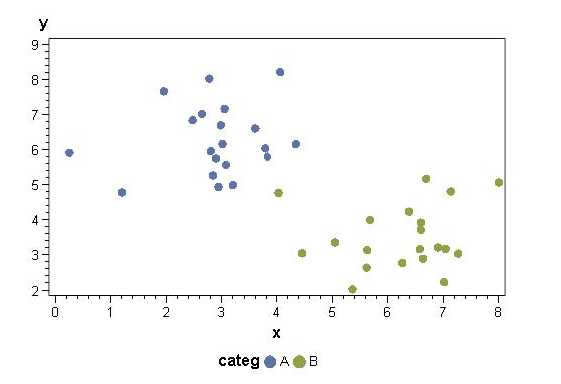
\includegraphics[width=\textwidth]{Stat_base}
	\end{frame}

	\begin{frame}
	\frametitle{Nouveau repère}
		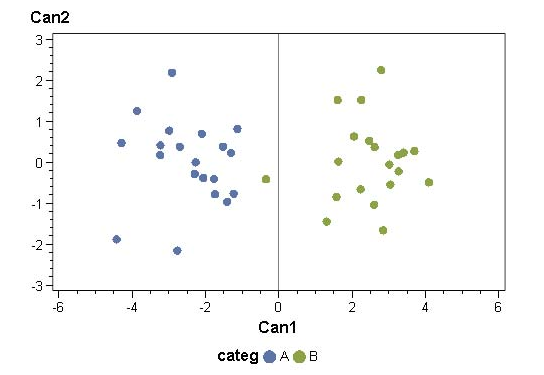
\includegraphics[width=\textwidth]{Stat_nouveau}
	\end{frame}
	\begin{frame}
		Mettre package utilisé avec la méthode discrimin + explications
	\end{frame}
	\section{Exemple}
	\begin{frame}
		Montrer exemple
	\end{frame}
\end{document}